\def\pgfsysdriver{pgfsys-dvisvgm.def}
% flashcards-title: Matter cycle and one-way energy path
% flashcards-desc: Solid green arrows loop among air, organism, and soil. Blue and orange arrows carry energy from light through the organism to heat leaving the system.
\documentclass[tikz,border=6pt]{standalone}
\usetikzlibrary{arrows.meta,calc,fit,positioning,shapes.geometric}

\definecolor{fcink}{HTML}{17212B}
\definecolor{fcblue}{HTML}{1D5D8C}
\definecolor{fcgreen}{HTML}{2D6A4F}
\definecolor{fcorange}{HTML}{A44A1F}
\definecolor{fcpale}{HTML}{F4F7F9}
\definecolor{fcsoil}{HTML}{8B5E3C}

\tikzset{
  fc text/.style={font=\sffamily, text=fcink},
  fc panel/.style={draw=fcink, line width=0.9pt, rounded corners=5pt, fill=fcpale},
  fc node/.style={draw=fcink, line width=0.9pt, rounded corners=4pt, fill=white,
    minimum width=24mm, minimum height=10mm, align=center, font=\sffamily},
  fc arrow/.style={-{Stealth[length=3.2mm,width=2.4mm]}, line width=1.2pt,
    draw=fcblue, line cap=butt},
  fc boundary/.style={draw=fcorange, line width=1.4pt, dash pattern=on 5pt off 3pt,
    rounded corners=7pt},
  fc label/.style={font=\sffamily\bfseries, text=fcink},
  fc note/.style={font=\sffamily\small, text=fcink, align=center}
}

\begin{document}
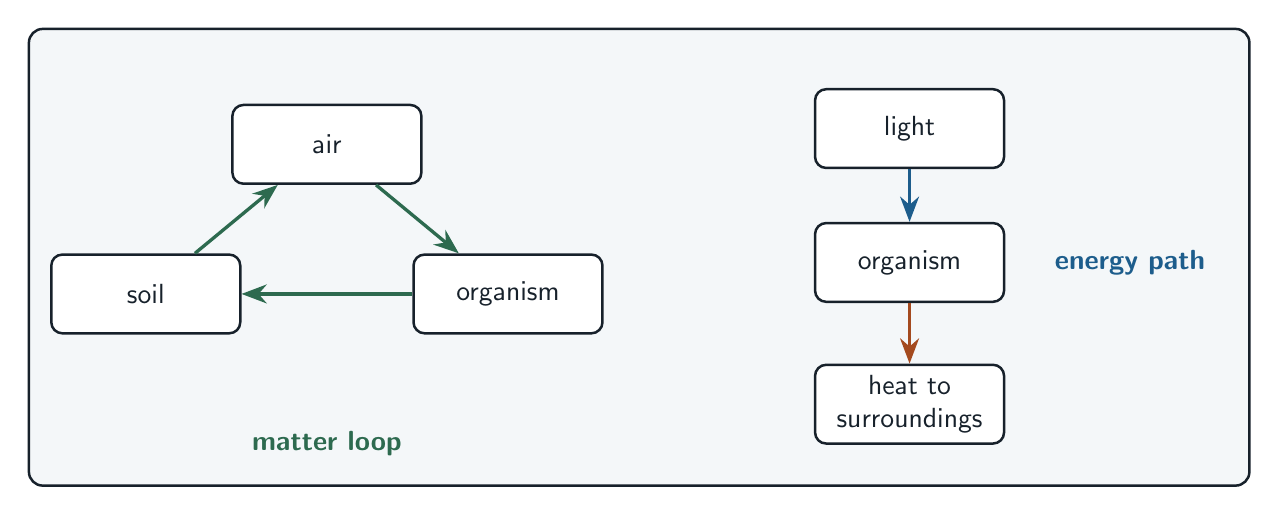
\begin{tikzpicture}[fc text, x=1cm, y=1cm]
  \node[fc panel, minimum width=155mm, minimum height=58mm, anchor=south west] at (0,0) {};
  \node[fc node] (air) at (3.8,4.35) {air};
  \node[fc node] (org) at (6.1,2.45) {organism};
  \node[fc node] (soil) at (1.5,2.45) {soil};
  \draw[fc arrow, draw=fcgreen] (air)--(org);
  \draw[fc arrow, draw=fcgreen] (org)--(soil);
  \draw[fc arrow, draw=fcgreen] (soil)--(air);
  \node[fc label, text=fcgreen] at (3.8,0.55) {matter loop};
  \node[fc node] (light) at (11.2,4.55) {light};
  \node[fc node] (use) at (11.2,2.85) {organism};
  \node[fc node] (heat) at (11.2,1.05) {heat to\\surroundings};
  \draw[fc arrow] (light)--(use);
  \draw[fc arrow, draw=fcorange] (use)--(heat);
  \node[fc label, text=fcblue] at (14.0,2.85) {energy path};
\end{tikzpicture}
\end{document}
